\documentclass{beamer}
%Information to be included in the title page:
% \title{Sample title}
% \author{Anonymous}
% \institute{Overleaf}
\usepackage{booktabs}
\usepackage{graphicx}
\usepackage[]{hyperref}

\usetheme[]{default}
\begin{document}
\renewcommand{\d}{\: \mathrm{d} }
\newcommand{\e}{\mathrm{e}}


\title[] {Recitation Class 2}

\author[lzx]{Zexi Li}

\institute[email]{lzx12138@sjtu.edu.cn}

\date{2021.05.25}

\frame{\titlepage}

\AtBeginSection[]
{
  \begin{frame}
    \frametitle{Table of Contents}
    \tableofcontents[currentsection]
  \end{frame}
}

\begin{frame}
    \frametitle{Outline}
    \tableofcontents
\end{frame}

% https://eng.libretexts.org/Bookshelves/Materials_Science/Supplemental_Modules_(Materials_Science)/Electronic_Properties/Density_of_States

\section{Chapter 3-II Introduction to the Quantum Theory of Solids}
    \begin{frame} \frametitle{Effective Mass: experimentally}
        Cyclotron resonance
        \begin{figure}[H]
            \centering
            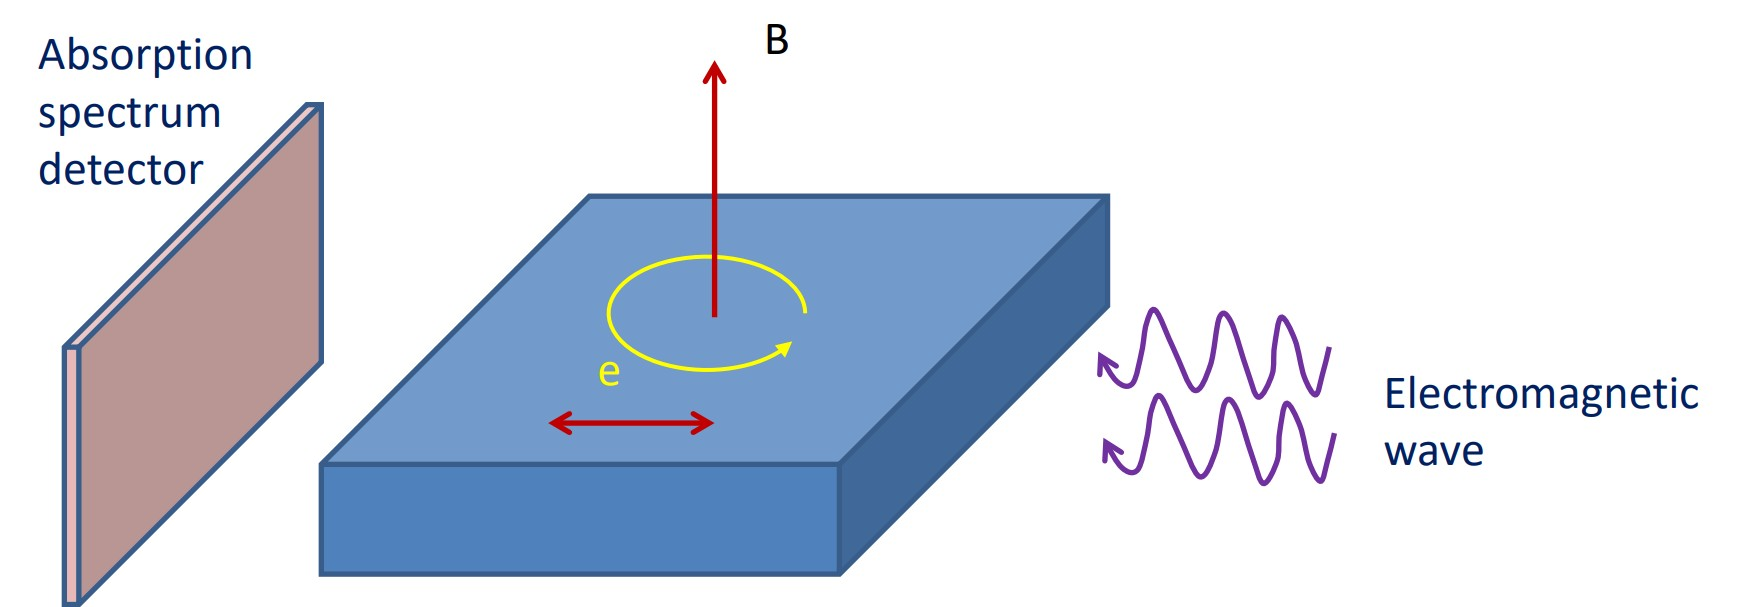
\includegraphics[width=0.6\linewidth]{Effective-mass-experiment.jpg}
            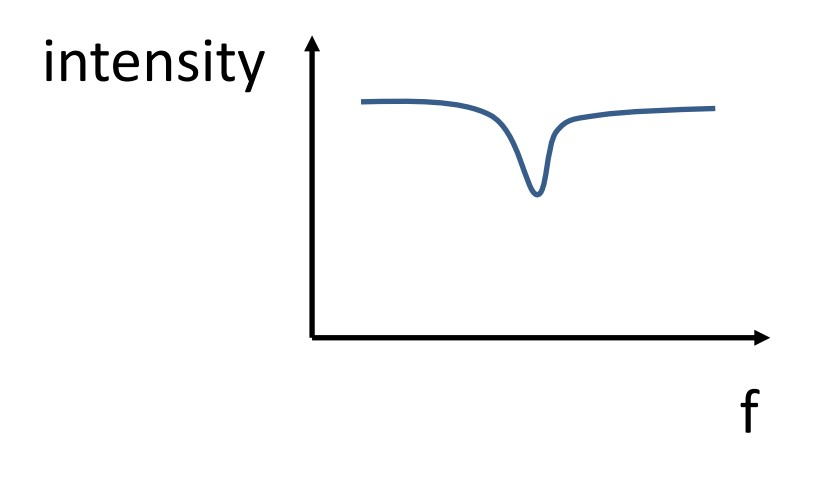
\includegraphics[width=0.3\linewidth]{Effective-mass-experiment-graph.jpg}
            \label{fig:Effective-mass-experiment.jpg}
        \end{figure}
        \begin{equation*}
            \boxed{m^* = \frac{eB\lambda}{2\pi c} }
        \end{equation*}
    \end{frame}

    \begin{frame} \frametitle{Density of States Function}
        \begin{figure}[H]
            \centering
            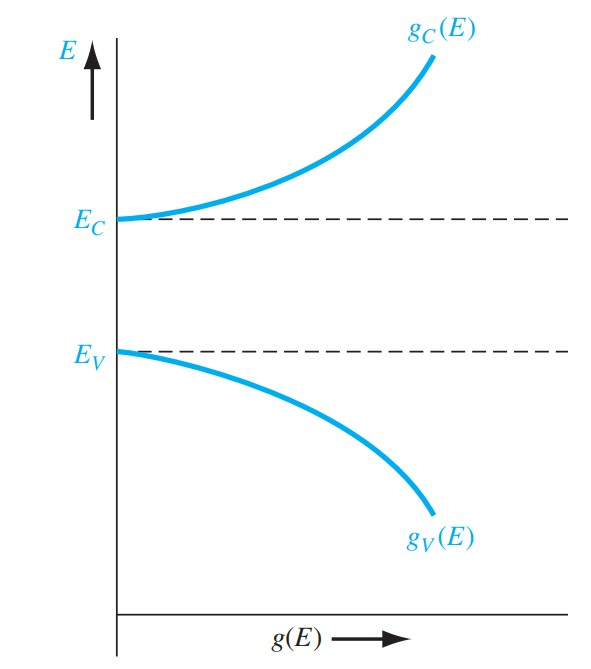
\includegraphics[width=0.3\linewidth]{Density-state-function.jpg}
            \label{fig:Density-state-function.jpg}
        \end{figure}
        \begin{equation*}
            \boxed{
                \begin{aligned}
                    g(E) &= \frac{4 \pi (2m)^{\frac{3}{2} }}{h^3} \sqrt{E}  \\
                    g_c(E) &= \frac{4 \pi (2m_n^*)^{\frac{3}{2} }}{h^3} \sqrt{E - E_c}  \\
                    g_v(E) &= \frac{4 \pi (2m_p^*)^{\frac{3}{2} }}{h^3} \sqrt{E_v - E}  \\
                \end{aligned}
            }
        \end{equation*}
    \end{frame}

    \begin{frame} \frametitle{Related Materials}
        Proof (if interested):
        \begin{itemize}
            \item \url{https://eng.libretexts.org/Bookshelves/Materials\_Science/Supplemental\_Modules\_(Materials\_Science)/Electronic\_Properties/Density\_of\_States}
            \item Textbook 3.4 Density of States Function
        \end{itemize}
    \end{frame}

    \begin{frame} \frametitle{Example}
        \par Determine the number (\#/cm$^3$) of quantum states in silicon between $E_c$ and $E_c + kT$ at $T = 300K$.

        \begin{equation*}
            \begin{aligned}
                N &= \int_{E_c}^{E_c + kT} \frac{4\pi (2m^*)^{3/2}}{h^3} \sqrt{E - E_c} \d E  \\
                &= \frac{4\pi (2m^*)^{3/2}}{h^3} \frac{2}{3} \left. (E - E_c)^{3/2} \right|_{E_c}^{E_c + kT} \\
                &= 2.22 \times 10^{25} m^{-3}\text{ or } 2.12 \times 10^{19} cm^{-3}
            \end{aligned}
        \end{equation*}

    \end{frame}

    \begin{frame} \frametitle{Distribution Function}
        \begin{itemize}
            \item Fermi-Dirac probability function:
                \begin{equation*}
                    f_F(E) = \frac{1}{1 + \exp\left( \frac{E - E_F}{kT}  \right)} 
                \end{equation*}
                \begin{figure}[H]
                    \centering
                    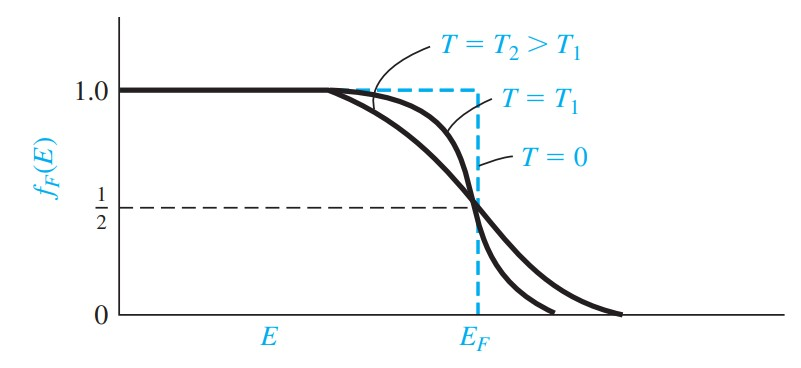
\includegraphics[width=0.8\linewidth]{Fermi-distribution.jpg}
                    \label{fig:Fermi-distribution.jpg}
                \end{figure}
        \end{itemize}
    \end{frame}

    \begin{frame} \frametitle{Distribution Function}
        \begin{itemize}
            \item Boltzmann distribution
                \par When $\exp \left( \frac{E - E_F}{kT} \right) >> 1 \Rightarrow E - E_F > 2kT$
                \begin{equation*}
                    f_F(E) \approx exp\left( -\frac{E - E_F}{kT}  \right)
                \end{equation*}
                \begin{figure}[H]
                    \centering
                    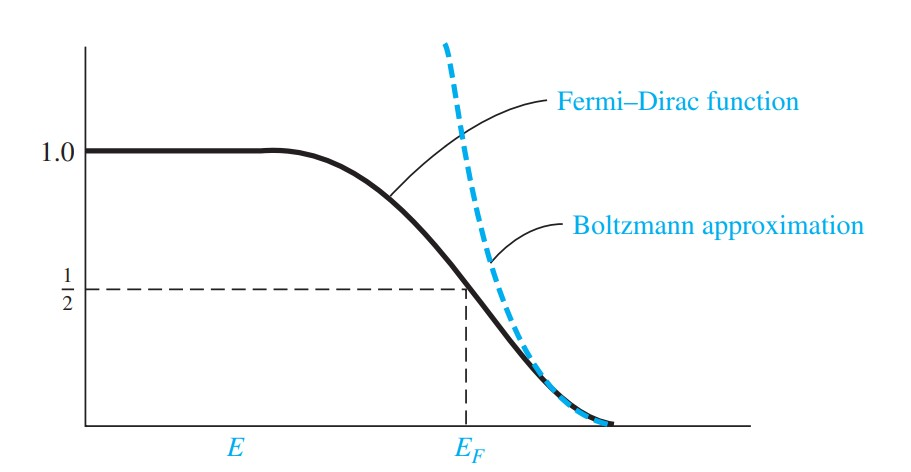
\includegraphics[width=0.8\linewidth]{Boltzmann-distribution.jpg}
                    \label{fig:Boltzmann-distribution.jpg}
                \end{figure}
        \end{itemize}
    \end{frame}


\section{Chapter 4-I The Semiconductor in Equilibrium}
    \begin{frame} \frametitle{$n_0$ and $p_0$ Equations}
        \begin{equation*}
            \begin{aligned}
                &n_0 = \int_{E_c}^\infty g_c(E) f_F(E) \d E \\
                \Rightarrow \quad &\boxed{n_0 = N_c \exp \left[ \frac{-(E_c - E_F)}{kT}  \right], \quad N_c = 2 \left( \frac{2\pi m_n^* kT}{h^2}  \right)^{3/2}} \\
                &p_0 = \int_{-\infty}^{E_v} g_v(E) \left(1 - f_F(E)\right) \d E \\
                \Rightarrow \quad &\boxed{p_0 = N_v \exp\left[ \frac{-(E_F - E_v)}{kT}  \right], \quad N_v = 2 \left( \frac{2\pi m_p^* kT}{h^2}  \right)^{3/2}}
            \end{aligned}
        \end{equation*}
    \end{frame}

    \begin{frame} \frametitle{Example}
        \par Calculate the thermal-equilibrium hole concentration in silicon at $T = 400K$. Assume that the Fermi energy is $0.27eV$ above the valence-band energy. The value of $N_v$ for silicon at $T = 300K$ is $N_v = 1.04 \times 10^{19} cm^{-3}$.
        \vspace{2em}
        \begin{center}
            \underline{$kT = 0.0259$ only for $T = 300K$}
        \end{center}
        \begin{equation*}
            \begin{aligned}
                &kT = (0.0259) \left( \frac{400}{300}  \right) = 0.03453 eV\\
                &N_v = (1.04 \times 10^{19}) \left( \frac{400}{300}  \right)^{3/2} = 1.60 \times 10^{19} cm^{-3}
            \end{aligned}
        \end{equation*}
        The hole concentration is then 
        \begin{equation*}
            \begin{aligned}
                p_0 = N_v \exp \left[ \frac{- (E_F - E_v)}{kT}  \right] &= (2.60 \times 10^{19}) \exp\left( \frac{-0.27}{0.03453}  \right) \\ &= 6.43 \times 10^{15} cm^{-3}
            \end{aligned}
        \end{equation*}
    \end{frame}

    \begin{frame} \frametitle{Intrinsic Semiconductor}
        For intrinsic semiconductor, the Fermi energy level is called the intrinsic Fermi energy, or $E_F = E_{Fi}$. We have
        \begin{equation*}
            \begin{aligned}
                n_0 &= n_i = N_c \exp \left[ \frac{-(E_c - E_{Fi})}{kT}\right] \\
                p_0 &= n_i = N_v \exp \left[ \frac{-(E_{Fi} -E_v)}{kT}  \right]
            \end{aligned}
        \end{equation*}
        Take the product:
        \begin{equation*}
            \boxed{n_0 p_0 = n_i^2 = N_cN_v \exp \left[ \frac{-(E_c - E_v)}{kT}  \right] = N_c N_v \exp \left[ \frac{-E_g}{kT}  \right]}
        \end{equation*}
    \end{frame}

    \begin{frame}[t] \frametitle{Self-consistency}
        \begin{equation*}
            n_i^2 = N_cN_v \exp \left[ \frac{-(E_c - E_v)}{kT}  \right] = N_c N_v \exp \left[ \frac{-E_g}{kT}  \right]
        \end{equation*}
        \vspace{2em}
        \par For $Si$ at $300K$:
        \begin{equation*}
            \begin{aligned}
                &n_i = 1.5 \times 10^{10} cm^{-3},\\ &E_g = 1.12 eV, \\ 
                &N_c = 2.8 \times 10^{19} cm^{-3},\\ &N_v = 1.04 \times 10^{19} cm^{-3},\\ &kT = 0.0259 eV
            \end{aligned}
        \end{equation*}
        \begin{equation*}
            LHS = 2.25 \times 10^{20} {\color{red} \neq } 4.82936 \times 10^{19} = RHS  
        \end{equation*}
    \end{frame}

    \begin{frame} \frametitle{Self-consistency Example}
        For n-doped Silicon semiconductor at $300K$, the Fermi level is $E_F = E_c - 0.3eV$. Calculate $p_0$.
        \begin{itemize}
            \item Approach I:
                \begin{equation*}
                    \begin{aligned}
                        n_0 &= N_c \exp \left[ \frac{-(E_c - E_F)}{kT}  \right] = 2.61 \times 10^{14} cm^{-3}\\
                        p_0 &= \frac{n_i^2}{n_0} = 8.62 \times 10^{5} cm^{-3}
                    \end{aligned}
                \end{equation*}
            \item Approach II:
                \begin{equation*}
                    \begin{aligned}
                        &E_F - E_v = E_g - (E_c - E_F) = 0.82 eV \\
                        &p_0 = N_v \exp\left[ \frac{-(E_F - E_v)}{kT}  \right] = 1.85 \times 10^5 cm^{-3}
                    \end{aligned}
                \end{equation*}
        \end{itemize}
    \end{frame}

    \begin{frame} 
        \begin{center}
            \Large\textcolor{blue}{End}
        \end{center}
    \end{frame}
\end{document}